% Settings
\ifEMBED
    \setcounter{tocdepth}{4}   %= Aufnahme in das Inhaltsverzeichnis *
    \setcounter{secnumdepth}{4}  % = Nummerierung vertiefen *
\fi

% title page
\ifSTANDALONE
    \ifDC
        \begin{titlepage}

\begin{center}

% Oberer Teil der Titelseite:
%\includegraphics[width=0.15\textwidth]{./logo}\\[1cm]    
\textsc{\LARGE Produktentwicklung 1}\\[1.5cm]

\textsc{\Large Hochschule Luzern\\
    ~\\
    Technik \& Architektur}\\[0.5cm]

\vfill{}

% Title
\newcommand{\HRule}{\rule{\linewidth}{0.5mm}}
\HRule \\[0.4cm]
{   \Huge \bfseries DC Treiber\\
        ~\\
        \large Konzeptbeschreibung}\\[0.4cm]

\HRule \\[1.5cm]

% Author and supervisor
\begin{minipage}{0.4\textwidth}
    \begin{flushleft} \large
        \emph{Autoren:}\\
        Ervin \textsc{Mazlagi\'c}\\
        Flavio \textsc{Kreiliger}\\
    \end{flushleft}
\end{minipage}
\hfill
\begin{minipage}{0.4\textwidth}
    \begin{flushright} \large
        \emph{Projektgruppe:} \\
        PREN-ET
    \end{flushright}
\end{minipage}

\vfill{}
\vfill{}
\vfill{}

% Unterer Teil der Seite
{\large Horw\\ \today}

\end{center}

\end{titlepage}

    \fi
    \ifBLDC
        \begin{titlepage}

\begin{center}

% Oberer Teil der Titelseite:
%\includegraphics[width=0.15\textwidth]{./logo}\\[1cm]    
\textsc{\LARGE Produktentwicklung 1}\\[1.5cm]

\textsc{\Large Hochschule Luzern\\
    ~\\
    Technik \& Architektur}\\[0.5cm]

\vfill{}

% Title
\newcommand{\HRule}{\rule{\linewidth}{0.5mm}}
\HRule \\[0.4cm]
{   \Huge \bfseries Brushless DC Treiber\\
        ~\\
        \large Konzeptbeschreibung}\\[0.4cm]

\HRule \\[1.5cm]

% Author and supervisor
\begin{minipage}{0.4\textwidth}
    \begin{flushleft} \large
        \emph{Autoren:}\\
        Yves \textsc{Studer}\\
        Daniel \textsc{Winz}\\
        Ervin \textsc{Mazlagi\'c}\\
    \end{flushleft}
\end{minipage}
\hfill
\begin{minipage}{0.4\textwidth}
    \begin{flushright} \large
        \emph{Projektgruppe:} \\
        PREN-ET
    \end{flushright}
\end{minipage}

\vfill{}
\vfill{}
\vfill{}

% Unterer Teil der Seite
{\large Horw\\ \today}

\end{center}

\end{titlepage}

    \fi
    \ifSTEPPER
        \begin{titlepage}

\begin{center}

% Oberer Teil der Titelseite:
%\includegraphics[width=0.15\textwidth]{./logo}\\[1cm]    
\textsc{\LARGE Produktentwicklung 1}\\[1.5cm]

\textsc{\Large Hochschule Luzern\\
    ~\\
    Technik \& Architektur}\\[0.5cm]

\vfill{}

% Title
\newcommand{\HRule}{\rule{\linewidth}{0.5mm}}
\HRule \\[0.4cm]
{   \Huge \bfseries Stepper Treiber\\
        ~\\
        \large Konzeptbeschreibung}\\[0.4cm]

\HRule \\[1.5cm]

% Author and supervisor
\begin{minipage}{0.4\textwidth}
    \begin{flushleft} \large
        \emph{Autorin:}\\
        Bettina \textsc{Wyss}\\
    \end{flushleft}
\end{minipage}
\hfill
\begin{minipage}{0.4\textwidth}
    \begin{flushright} \large
        \emph{Projektgruppe:} \\
        PREN-ET
    \end{flushright}
\end{minipage}

\vfill{}
\vfill{}
\vfill{}

% Unterer Teil der Seite
{\large Horw\\ \today}

\end{center}

\end{titlepage}

    \fi
\else
    \author{PREN-ET}
    \maketitle
\fi

% Content
\tableofcontents
\clearpage
\ifSTANDALONE
\section{Hardware}
\fi
\ifEMBED
\subsection{Hardware}
\fi
Die Elektrotechnik-Studierenden aus mehreren Gruppen haben sich
zusammengeschlossen um gemeinsame Probleme anzugehen. Dabei handelt es sich
um die benötigte Hard- und Software, um Motoren anzusteuern
und gegebenenfalls zu regeln. In diesem Zusammenschluss wurden drei Gruppen
gebildet, um Lösungen für DC-, Stepper- und Brushless-Motoren auszuarbeiten.
Die Idee besteht darin, dass nicht jede Gruppe für dasselbe Problem wo
möglich denselben Lösungsansatz verfolgt, sondern die Ressourcen kombiniert,
Synergien nutzt um eine bessere Lösung zu erarbeiten. Auf diese Weise kann
das Team übergreifende Arbeiten im Rahmen der PREN erlernt und
geübt werden. Somit wird Idee der Interdisziplinarität im erweiterten Sinn
Rechnung getragen. Die Gruppen und deren Mitglieder sind in der Tabelle 
\ref{tab:pren-et-overview} aufgeführt.
\begin{table}[h!]
	\centering
	\begin{tabular}{l l}
		Projekt		& Team \\
		\hline
		DC Motoren	& 39 \\
		Schrittmotor	& 27, 38 \\
		BLDC Motor	& 27, 32 \\
	\end{tabular}
	\caption{Übersicht der PREN-ET Projektgruppen}
	\label{tab:pren-et-overview}
\end{table}

\ifDC
    \renewcommand{\EtPath}{src/DC}
    \ifSTANDALONE
\section{Konzept}
\fi
\ifEMBED
\subsection{Konzept}
\fi

Das Stellen eines fremderregten Gleichstrommotors erfolgt über die
angelegte Ankerspannung. Eine variable Ankerspannung kann mittels einer 
zeitlichen Mittelung der anliegenden Spannung realisert werden. Somit
ist es möglich eine fremderregte Gleichstrommaschine mittels einer
konstanten Gleichspannung einzustellen. Die Mittelung der Ankerspannung
bildet die Basis des vorliegenden Konzepts für den DC-Motor Treiber.

\ifSTANDALONE
\subsection{Annahmen und Abschätzungen}\label{sec:annahmen}
\fi
\ifEMBED
\subsubsection{Annahmen und Abschätzungen}\label{sec:annahmen}
\fi
Für das vorliegende Konzept gilt die Annahme, dass das Erregerfeld mittels
Permanentmagneten realisiert ist und das Erregerfeld konstant ist. Diese
Annahme ist gewählt, da fremderregte Gleichstrommaschinen ohne
Permanentmagneten einen Erregerstrom benötigen, welcher das Erregerfeld
erzeugt. Im einfachsten Fall ist dies eine Kosntantstromquelle. Eine solche
Maschine benötigt mehr elektrische Energie und erfordert zusätzlichen
Hardwareaufwand.

Die Drehzahl einer idealen fremderregten Gleichstrommaschine mit konstantem
Erregerfeld korreliert mit $-1$ zum Strom. Der Strom einer solchen Maschine
korreliert widerum mit der Belastung \cite[p.163]{smps}. Dieses Verahalten
zwischen Belastung und Drehzahl ist in Abbildung \ref{fig:ideal-dc-curve}
dargestellt.

\begin{figure}[h!]
	\centering
	\begin{tikzpicture}
		% Achsen
		\draw[->] (-0.5,0) -- (8,0) node[anchor=north] {$I, M$};
		\draw[->] (0,-0.5) -- (0,4) node[anchor=east] {$\omega_m$};
		% Klemmenspannung
		\draw[blue, thick] (0,3) -- (7,3) node[anchor=west] {$U_K$};
		% induzierte Spannung
		\draw[red, thick] 
			(0,3) node[anchor=east] {$\omega_0$} -- 
			(7,0) node[midway, above right] {$\omega \sim U_i$};
		
	\end{tikzpicture}
	\caption{Winkelgeschwindigkeit einer idealen fremderregten 
		Gleichstrommaschine}
	\label{fig:ideal-dc-curve}
\end{figure}

\ifSTANDALONE
\subsection{Ziel}
\fi
\ifEMBED
\subsubsection{Ziel}
\fi
Es ist eine Hardware zu entwicklen, welche es ermöglicht, die
Winkelgeschwindigkeit einer fremerregten Gleichstrommaschine mit
Permanentmagneten zu regeln.

\ifSTANDALONE
\subsection{Funktionsweise}
\fi
\ifEMBED
\subsubsection{Funktionsweise}
\fi
Um die Klemmenspannung der Gleichstrommaschine zu stellen, wird eine
H-Brücke verwendet. Diese kann je nach Bedarf individuell ausgelegt
werden. Die Ansteuerung der H-Brücke erfolgt mittels des Treiberschips
A3941 von Allegro Microsystems. Das Interfaces, welches der
Treiberchip zur Verfügung stellt, wird mittels eines Mikrocontrollers
bedient, welcher ebenfalls individuell gewählt ist.

\begin{figure}[h!]
	\centering
	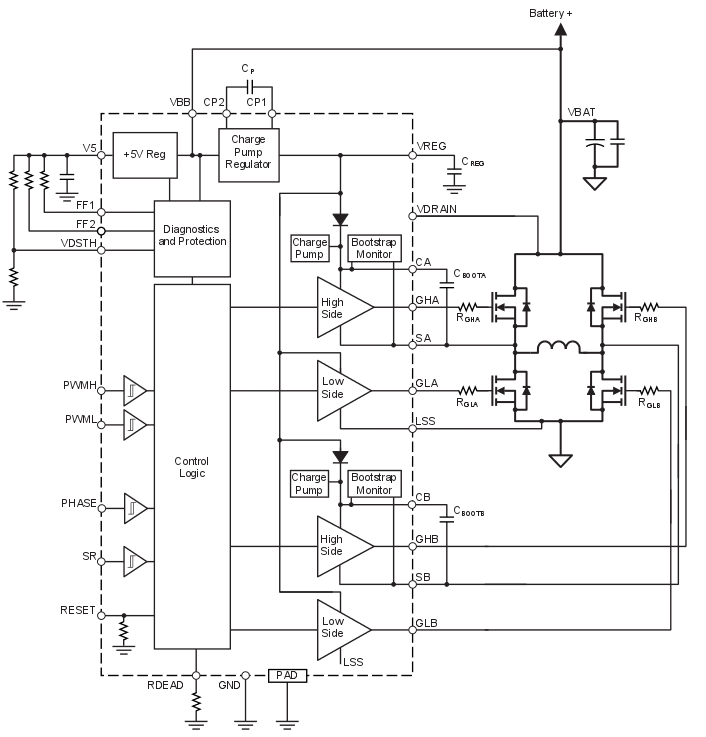
\includegraphics[width=0.75\textwidth]{src/DC/fig/a3941-functional.png}
	\caption{Blockaschltbild des A3941}
	\label{fig:a3941-functional}
\end{figure}

Die Regelung der Winkelgeschwindigkeit eines angeschlossenen Motors kann
mit verschiedenen Ansätzen realisert werden. Gemeinsam ist dabei stets die
Stellgrösse, welche durch das PWM Signal gegeben ist, als auch die
Winkelgeschwindigkeit der Maschine, welche die Regelgrösse darstellt.

Die Regelung muss auf einem Feedback der Winkelgeschwindigkeit basieren.
Wird von einer idealen Maschine ausgegangen, muss dieses Feedback nicht
zwingend durch einen Encoder generiert werden, sondern kann implizit durch
den Strom gegeben sein, wie in der Abbildung \ref{fig:ideal-dc-curve}
dargestellt. Mit den getroffenen Annahmen aus dem Abschnitt
\ref{sec:annahmen} kann somit auf ein explizites Feedback der
Winkelgeschwindigkeit verzichtet werden. 

\ifSTANDALONE
\subsection{Regelung}
\fi
\ifEMBED
\subsubsection{Regelung}
\fi
Für die Ansteuerung der H-Brücke bzw. des Treiberchips A3941 wird ein PWM
Signal benötigt. Dieses kann in Hardware auf dem Treiberboard implementiert
werden mittels eines Sägezahngenerators und einem Komparator. Der zweite
Komparatoreingang wird dazu an das Feedback des Stromes angeschlossen, was
ein zur Winkelgeschwindigkeit angepasstes PWM Signal generiert.

Alternativ zu dieser Regelung kann das Feedbcak des Stromes auch zum
Mikrocontroller geführt werden, welcher dieses auswertet und ein passendes
PWM Signal generiert.

\begin{figure}[h!]
	\centering
	\begin{subfigure}[b]{0.45\textwidth}
		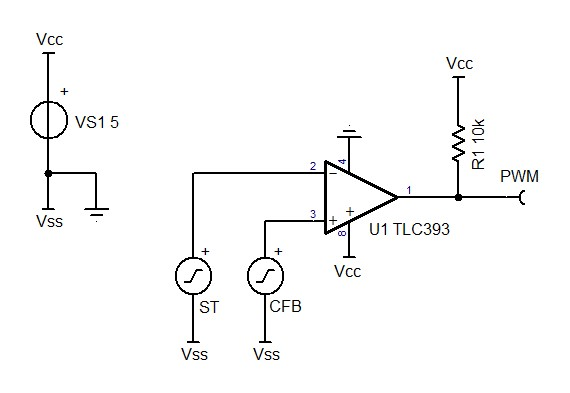
\includegraphics[width=\textwidth]{src/DC/sim/sch-pwm-01.jpg}
		\caption{Prinzipschema mit dem Komparator TLC393}
	\end{subfigure}
	\begin{subfigure}[b]{0.45\textwidth}
		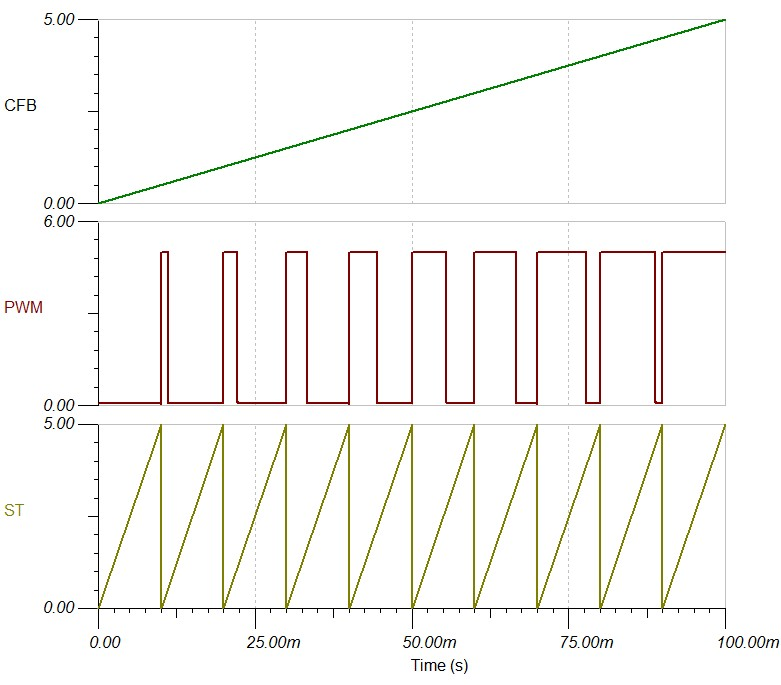
\includegraphics[width=\textwidth]{src/DC/sim/pwm-01.jpg}
		\caption{Simulationsergebnisse für lineares Feedback}
	\end{subfigure}
	\caption{Simulation eines PWM-Generator mit Komparator}
\end{figure}

\begin{figure}[h!]
	\centering
	\begin{subfigure}[b]{0.45\textwidth}
		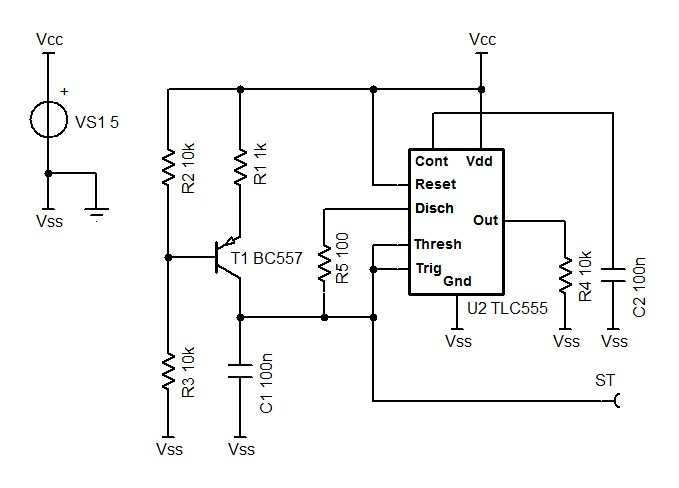
\includegraphics[width=\textwidth]{src/DC/sim/sch-sawtooth-01.jpg}
		\caption{Sägezahntgenerator mit Timer TLC555}
	\end{subfigure}
	\begin{subfigure}[b]{0.45\textwidth}
		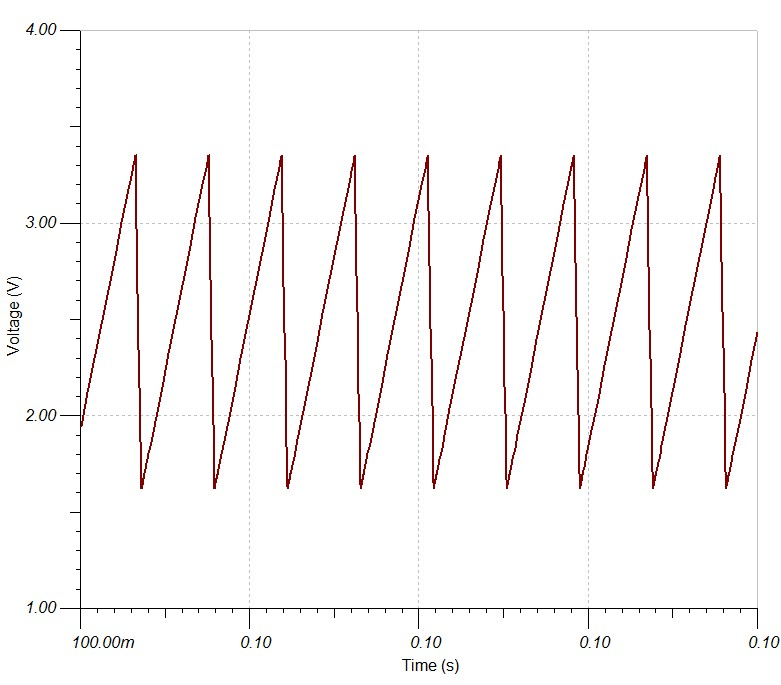
\includegraphics[width=\textwidth]{src/DC/sim/sawtooth-01.jpg}
		\caption{Simulationsergebnisse ($f_{ST} \approx 9.3$kHz)}
	\end{subfigure}
	\caption{Simulation eines Sägezahngenerators}
	\label{fig:sawtooth}
\end{figure}

Ein passender Baustein zur Erzeugung ist der Timer TLC555, wie in der
Abbildung \ref{fig:sawtooth} dargestellt. Das Feedback des Stromes kann
dabei auf verschiedene Weise implementiert werden. Einerseits gibt es eine
kostengünstige Variante mittels dem Einsatz eines Shunt-Widerstands. Dieser
bietet im Idealfall ein lineares Varhalten. In der Realität führt der
Einfluss der Temperatur zu einer deutlichen nichtlinearität dieses
Messmittels. Eine Alternative zum Shunt-Widerstands bietet der Einsatz von
Hall-Effekt-Stromwandlern, welche den Strom linearisiert als Spannungssignal
ausgeben. Ein solcher Baustein ist der ACS712 der Allegro Microsystems,
welcher im SMD Format verfügbar ist bis zu einem Strom von 30A.

Ist eine genaue Drehzahl nicht von Bedeutung kann auf die Regelung der
Winkelgeschwindigkeit verzichtet werden. Dies gilt insbesondere, wenn eine
hohe Übersetzung vorliegt, welche verhindert, dass die Winkelgeschwindigkeit
der Gleichstrommaschine einbricht bei entsprechender Belastung. Für diesen
Fall kann das PWM fix eingestellt werden und lediglich mit einem Enable
Signal gearbeitet werden. Dies lässt sich mit einer logischen AND Funktion
realisieren für das PWM Signal. Eine mögliche Implementation ist in der
Abbildung \ref{fig:and} dargestellt.

\begin{figure}[h!]
	\centering
	\begin{subfigure}[b]{0.45\textwidth}
		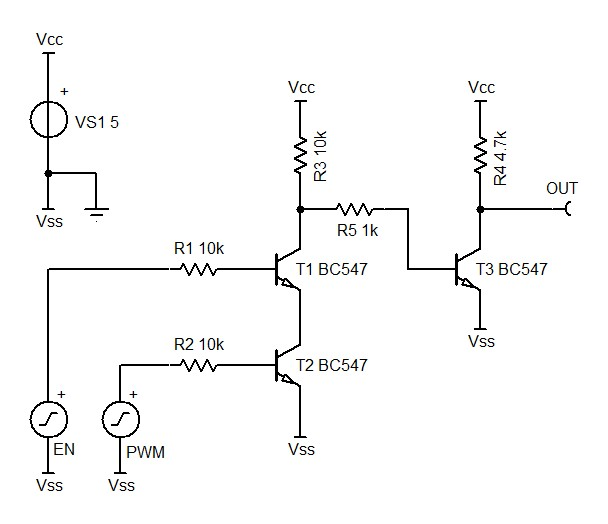
\includegraphics[width=\textwidth]{src/DC/sim/sch-and-01.jpg}
		\caption{AND-Schaltung mit NPN-Transistoren}
	\end{subfigure}
	\begin{subfigure}[b]{0.45\textwidth}
		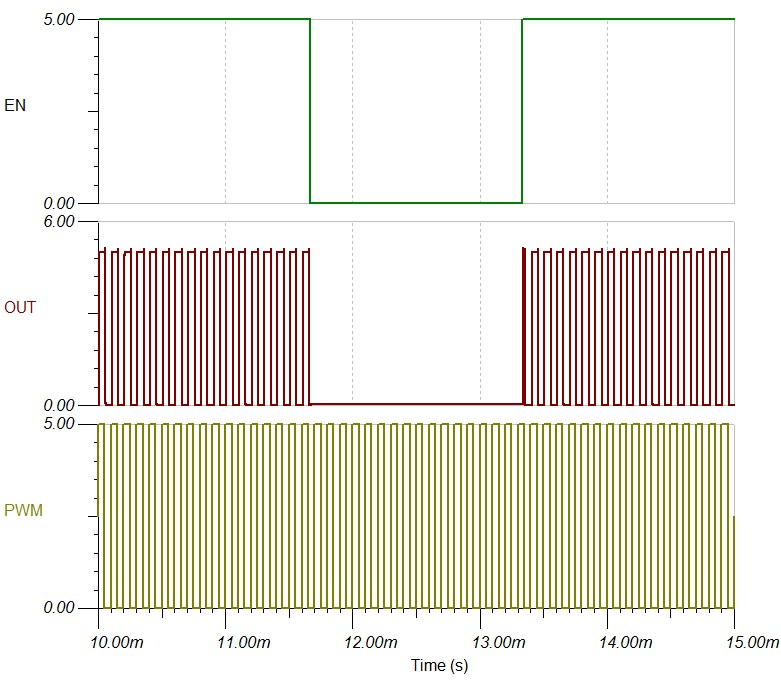
\includegraphics[width=\textwidth]{src/DC/sim/and-01.jpg}
		\caption{Simulationsergebnisse}
	\end{subfigure}
	\caption{Simulation einer AND-Schaltung realisiert mit
		Bipolartransistoren}
	\label{fig:and}
\end{figure}


    \newpage
\fi

\ifBLDC
    \renewcommand{\EtPath}{src/BLDC}
    \ifSTANDALONE
\section{Brushless Motoransteuerung}
\fi
\ifEMBED
\subsection{Brushless Motoransteuerung}
\fi

\ifEMBED
    % Dieses Kapitel ist eine Zusammenarbeit der Gruppen \BLDCTeams. 
    \BLDCcollab
\fi
    \ifSTANDALONE
    \subsection{Theorie der Ansteuerung}
    \fi
    \ifEMBED
    \subsubsection{Theorie der Ansteuerung}
    \fi
    \ifEMBED
        \begin{wrapfigure}{r}{0.50\textwidth}
           	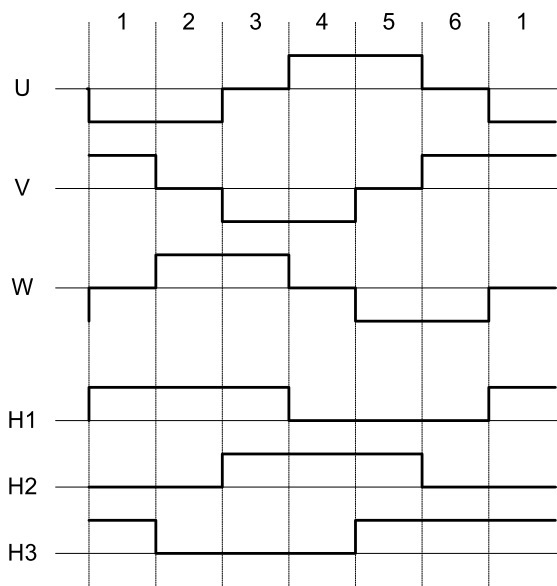
\includegraphics[scale=0.45]{\EtPath/Bilder/ZeitlicheHallSensorAnsteuerung.jpg}
           	\caption[Zeitliche Darstellung der Ansteuerung mit Hall-Sensoren]
           	{Zeitliche Darstellung der Ansteuerung mit Hall-Sensoren \cite{AppNote:BrushlessuC}}
           	\centering
            \label{abb:ZeitlicheAnsteuerungBrushlessMotor}
        \end{wrapfigure}
    \fi
        Brushless-Motoren (BLDC-Motoren) sind Synchron-Drehstrom-Motoren. Das bedeutet, sie
        werden mittels eines kontinuierlichen magnetischen Drehfeldes in Bewegung gesetzt.
        Dabei ist darauf zu achten, dass der Läufer dem Drehfeld synchron folgen kann,
        daher auch die Namensbezeichnung des Motors. Falls der Läufer dem Drehfeld nicht
        folgen kann, wird keine Spannung vom Rotor in die Statorwicklungen induziert, die
        der Erregerspannung entgegenwirkt. Daraus folgt, dass ein immenser Strom fliesst, 
        der nur von der Wicklungsimpedanz des Motors begrenzt wird.\\
        \ifSTANDALONE
           \begin{figure}[h!]
               \centering
               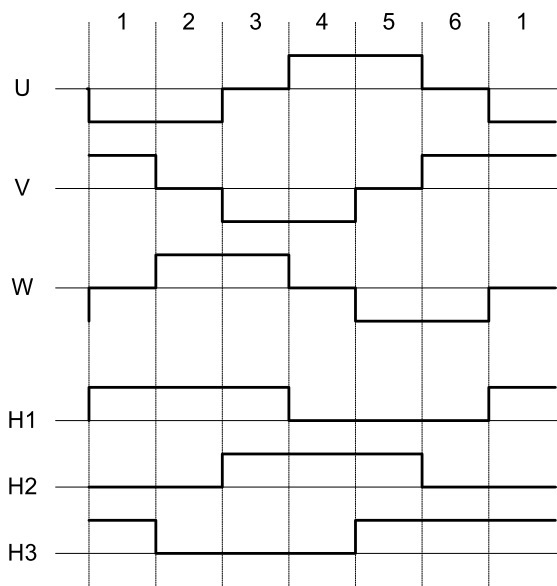
\includegraphics[scale=0.45]{\EtPath/Bilder/ZeitlicheHallSensorAnsteuerung.jpg}
               \caption[Zeitliche Darstellung der Ansteuerung mit 
                   Hall-Sensoren]{Zeitliche Darstellung der Ansteuerung mit 
                   Hall-Sensoren \cite{AppNote:BrushlessuC}}
              	\centering
               \label{abb:ZeitlicheAnsteuerungBrushlessMotor}
           \end{figure}
      \fi
       \\
        Es gibt hauptsächlich drei Methoden das Drehfeld zu generieren und zu 
        regeln. Die einfachste Methode ist die Zwangskommutierung: 
        Dabei wird ein Drehfeld erzeugt und dem Motor aufgezwungen. Der Läufer 
        muss dem Drehfeld folgen, der maximal zulässige Winkel von 90$^\circ$
        zwischen dem Feld und dem Läufer muss eingehalten werden. Wird dieser 
        Winkel überschritten, kommt der Motor zum Stillstand.\\
        \\
        Die zweite Methode zur Regelung des Motors verwendet drei Hallsensoren, die im 
        Motor integriert sind. Dies macht den Motor aufwändiger und 
        dementsprechend teurer. Die Regelung mit Hallsensoren ist 
        verhältnismässig einfach, da nach den Signalen die einzelnen Spulen 
        direkt angesteuert werden können. Der Zusammenhang zwischen der 
        Ansteuerung und den Hallsensor-Signalen ist in Abbildung 
        \ref{abb:ZeitlicheAnsteuerungBrushlessMotor} ersichtlich. Dabei stehen 
        $U$, $V$ und $W$ für die Phasenströme und $H_1$, $H_2$ und $H_3$ für die 
        entsprechenden Signale der Hallsensoren. Dieser Darstellung ist zu 
        entnehmen, wenn ein Hallsensor eine Änderung anzeigt, 
        ein Nulldurchgang im entsprechenden Stromverlauf stattgefunden hat. 
        Dies ist der Zeitpunkt, zu dem die Kommutierung durchgeführt werden 
        muss.\\
        \\
        Für die dritte Möglichkeit bildet man einen virtuellen Sternpunkt 
        und detektiert mit Komparatoren die Sternpunktdurchgänge. 
        In der Controller-Logik muss der Zeitunterschied der Kommutierung 
        bis zum durchschreiten des Sternpunktes gemessen werden. Diese Zeit 
        muss noch einmal abgewartet werden, bevor die Kommutierung durchgeführt 
        wird.
    \ifSTANDALONE
    \subsection{Neuer Ansatz}
    \fi
    \ifEMBED
    \subsubsection{Neuer Ansatz}
    \fi

        \ifEMBED
        \begin{wrapfigure}{r}{0.40\textwidth}
            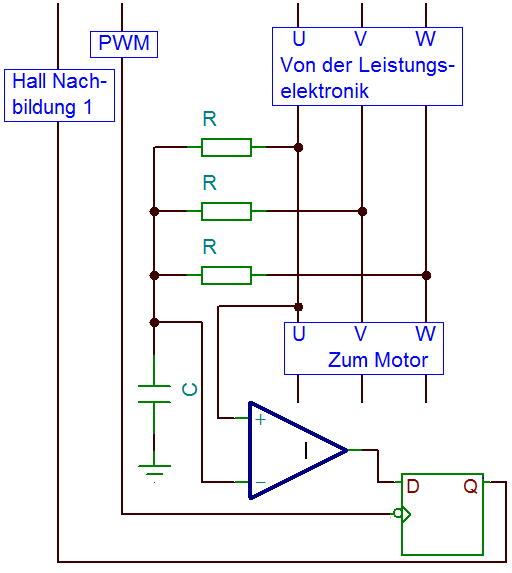
\includegraphics[scale=0.46]{\EtPath/Bilder/PrinzipDerRekonstruktion.png}
            \centering
            \caption[Schema des Rekonstruktionsprinzip]{Schema des Rekonstruktionsprinzip \cite{HSLU:Pluess}}
            \label{abb:PrinzipRekonstruktion}
            \end{wrapfigure}
        \fi
        In einem modifizierten Ansatz wird versucht, die Hallsensor-Signale 
        aus den Ansteuerungen des Motors zu gewinnen. Hierzu wird 
        eine Schaltung pro Phase benötigt, um die Nulldurchgänge beim 
        virtuellen Sternpunkt detektieren zu können. Die Abbildung 
        \ref{abb:PrinzipRekonstruktion} zeigt die Schaltung, mit der dieser Ansatz 
        realisiert werden kann. 
        \ifSTANDALONE
	\begin{figure}[h!]
            \centering
            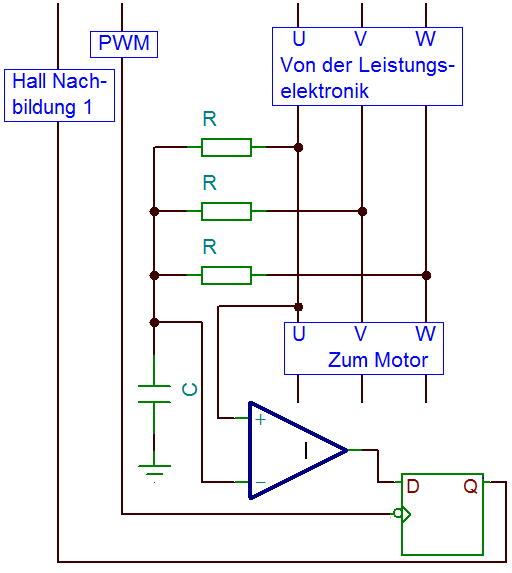
\includegraphics[scale=0.46]{\EtPath/Bilder/PrinzipDerRekonstruktion.png}
           	\caption{Schema des Rekonstruktionsprinzip \protect\cite{HSLU:Pluess}}
            \label{abb:PrinzipRekonstruktion}
        \end{figure}
        \fi
        Mit dem Flip-Flop aus Abbildung \ref{abb:PrinzipRekonstruktion} kann die PWM aus dem 
        Sensorsignal unterdrückt werden. Diese rekonstruierten 
        Hallsensor-Signale können direkt logisch verknüpft und genutzt 
        werden, um den Motor mit einer Dreiphasen-H-Brücke anzusteuern 
        \cite{HSLU:Pluess}. Anhand des zeitlichen Verlaufs, der aus Abbildung 
        \ref{abb:ZeitlicheAnsteuerungBrushlessMotor} zu entnehmen ist und der 
        Ansteuerung einer H-Brücke, ergibt sich die Wahrheitstabelle, die in 
        Abbildung \ref{abb:WahrheitstabelleAnsteuerung} ersichtlich ist. Das 
        Signal $U_h$ symbolisiert den Highside-Transistor der Phase U auf der 
        H-Brücke und die Spalte $U_l$ entspricht dem Lowside-Transistor.\\      
        
        \begin{figure}[h!]
            \begin{tabular}{ccc||cc|cc|cc||c}
                 $H_1$ & $H_2$ & $H_3$ & $U_h$ & $U_l$ & $V_h$ & $V_l$ & $W_h$ & $W_l$ & Illegal\\
            \hline 0   &   0   &   0   &   0   &   0   &   0   &   0   &   0   &   0   &   1\\
                   0   &   0   &   1   &   0   &   0   &   0   &   1   &   1   &   0   &   0\\
                   0   &   1   &   0   &   0   &   1   &   1   &   0   &   0   &   0   &   0\\
                   0   &   1   &   1   &   0   &   1   &   0   &   0   &   1   &   0   &   0\\
                   1   &   0   &   0   &   1   &   0   &   0   &   0   &   0   &   1   &   0\\
                   1   &   0   &   1   &   1   &   0   &   0   &   1   &   0   &   0   &   0\\
                   1   &   1   &   0   &   0   &   0   &   1   &   0   &   0   &   1   &   0\\
                   1   &   1   &   1   &   0   &   0   &   0   &   0   &   0   &   0   &   1\\
            \end{tabular}
           	\centering
           	\caption{Wahrheitstabelle der Ansteuerung} 
            \label{abb:WahrheitstabelleAnsteuerung}
        \end{figure}
        \parindent 0pt Die Tabelle in Abbildung 
        \ref{abb:WahrheitstabelleAnsteuerung} kann pro Signal zu folgenden 
        logischen Verknüpfung vereinfacht werden\\
        \\
        \ifSTANDALONE
        \begin{table}
            \centering
            \begin{tabular}{ccc}
                $U_h = H_1 \wedge \bar{H_2}$ & $V_h = H_2 \wedge \bar{H_3}$ & $W_h = \bar{H_1} \wedge H_3$\\
                $U_l = \bar{H_1} \wedge H_2$ & $V_l = \bar{H_2} \wedge H_3$ & $W_l = H_1 \wedge \bar{H_3}$
            \end{tabular}
        \end{table}
        \fi
        \ifEMBED
        \begin{tabular}{ccc}
            $U_h = H_1 \wedge \bar{H_2}$ & $V_h = H_2 \wedge \bar{H_3}$ & $W_h = \bar{H_1} \wedge H_3$\\
            $U_l = \bar{H_1} \wedge H_2$ & $V_l = \bar{H_2} \wedge H_3$ & $W_l = H_1 \wedge \bar{H_3}$
        \end{tabular}
        \fi

    \clearpage
    \ifSTANDALONE
\section{Prinziptest}
\fi
\ifEMBED
\subsubsection{Aufbaubeschreibung}
    \BLDCcollab
\fi
\ifEMBED
    \begin{wrapfigure}{r}{0.55\textwidth}
       	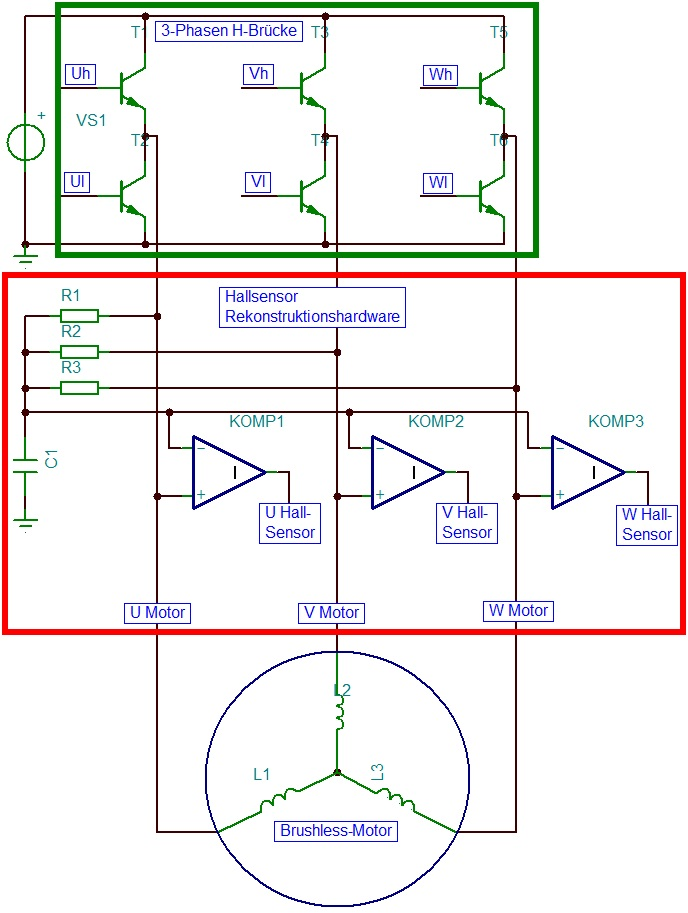
\includegraphics[scale=0.4]{\EtPath/Bilder/MotoransteuerungSchema.jpg}
       	\centering
       	\caption{Schema des Brushless-Versuchsaufbaus}
        \label{abb:MotoransteuerungSchema}
    \end{wrapfigure}
\fi
    Das Schema des Gesamtaufbaus des Tests ist in der Abbildung 
    \ref{abb:MotoransteuerungSchema} ersichtlich. Die 3-Phasen H-Brücke 
    im oberen grünen Rechteck wird direkt vom FPGA angesteuert. Die Hardware 
    dieser Brücke ermöglicht eine voll galvanisch getrennte Ansteuerung 
    mit 3.3V Logikpegeln. Diese Brücke wurde zur Verfügung gestellt und direkt
    implementiert. Die Rekonstruktion der Hallsensoren-Signale findet im rot 
    markierten Teil des Aufbaus statt. Dieser Part wurde auf einer 
    Laborplatte aufgebaut und gelötet. Die so generierten Signale 
    $U_{Hallsensor}$, $V_{Hallsensor}$, $W_{Hallsensor}$ werden einem FPGA 
    geliefert. Anhand dieser Signale steuert das FPGA die 
    H-Brücken-Transistoren mit den Signalen $U_h$, $U_l$, $V_h$, $V_l$, 
    $W_h$, $W_l$. Die im FPGA enthaltene Konfiguration besteht aus simplen 
    AND-Verknüpfungen, die die anliegenden Signale sehr schnell und 
    effizient verarbeiten können. Auf diese Weise ist es möglich, den Motor sehr 
    schnell anzusteuern.
    \ifSTANDALONE
    \begin{figure}[h!]
    	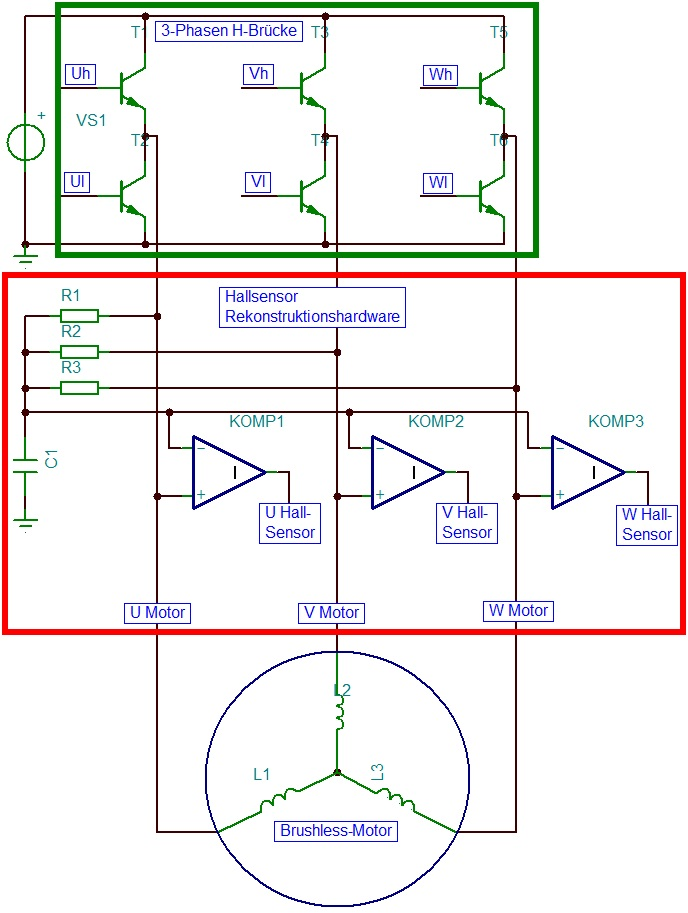
\includegraphics[scale=0.4]{\EtPath/Bilder/MotoransteuerungSchema.jpg}
       	\centering
       	\caption{Schema des Brushless-Versuchsaufbaus}
        \label{abb:MotoransteuerungSchema}
    \end{figure}
    \fi
    In der Abbildung \ref{abb:MessplatzAufbau} ist der gesamte Aufbau 
    abgebildet. Man beachte die markierten Felder. Am linken unteren Rand 
    ist der Motor befestigt. In der Mitte des Bildes ist die Hardware zur Rekonstruktion der Hallsensoren-Signale.
    Die generierten Signale werden dem FPGA in der unteren linken Ecke zugeführt. Diese 
    Signale werden logisch verknüpft und danach die sechs Signale 
    generiert, um die H-Brücke in der rechten oberen Hälfte anzusteuern. 
    Die H-Brücken wiederum treiben den Motor an.
    \begin{figure}[h!]
    %\vspace{-16pt}
       	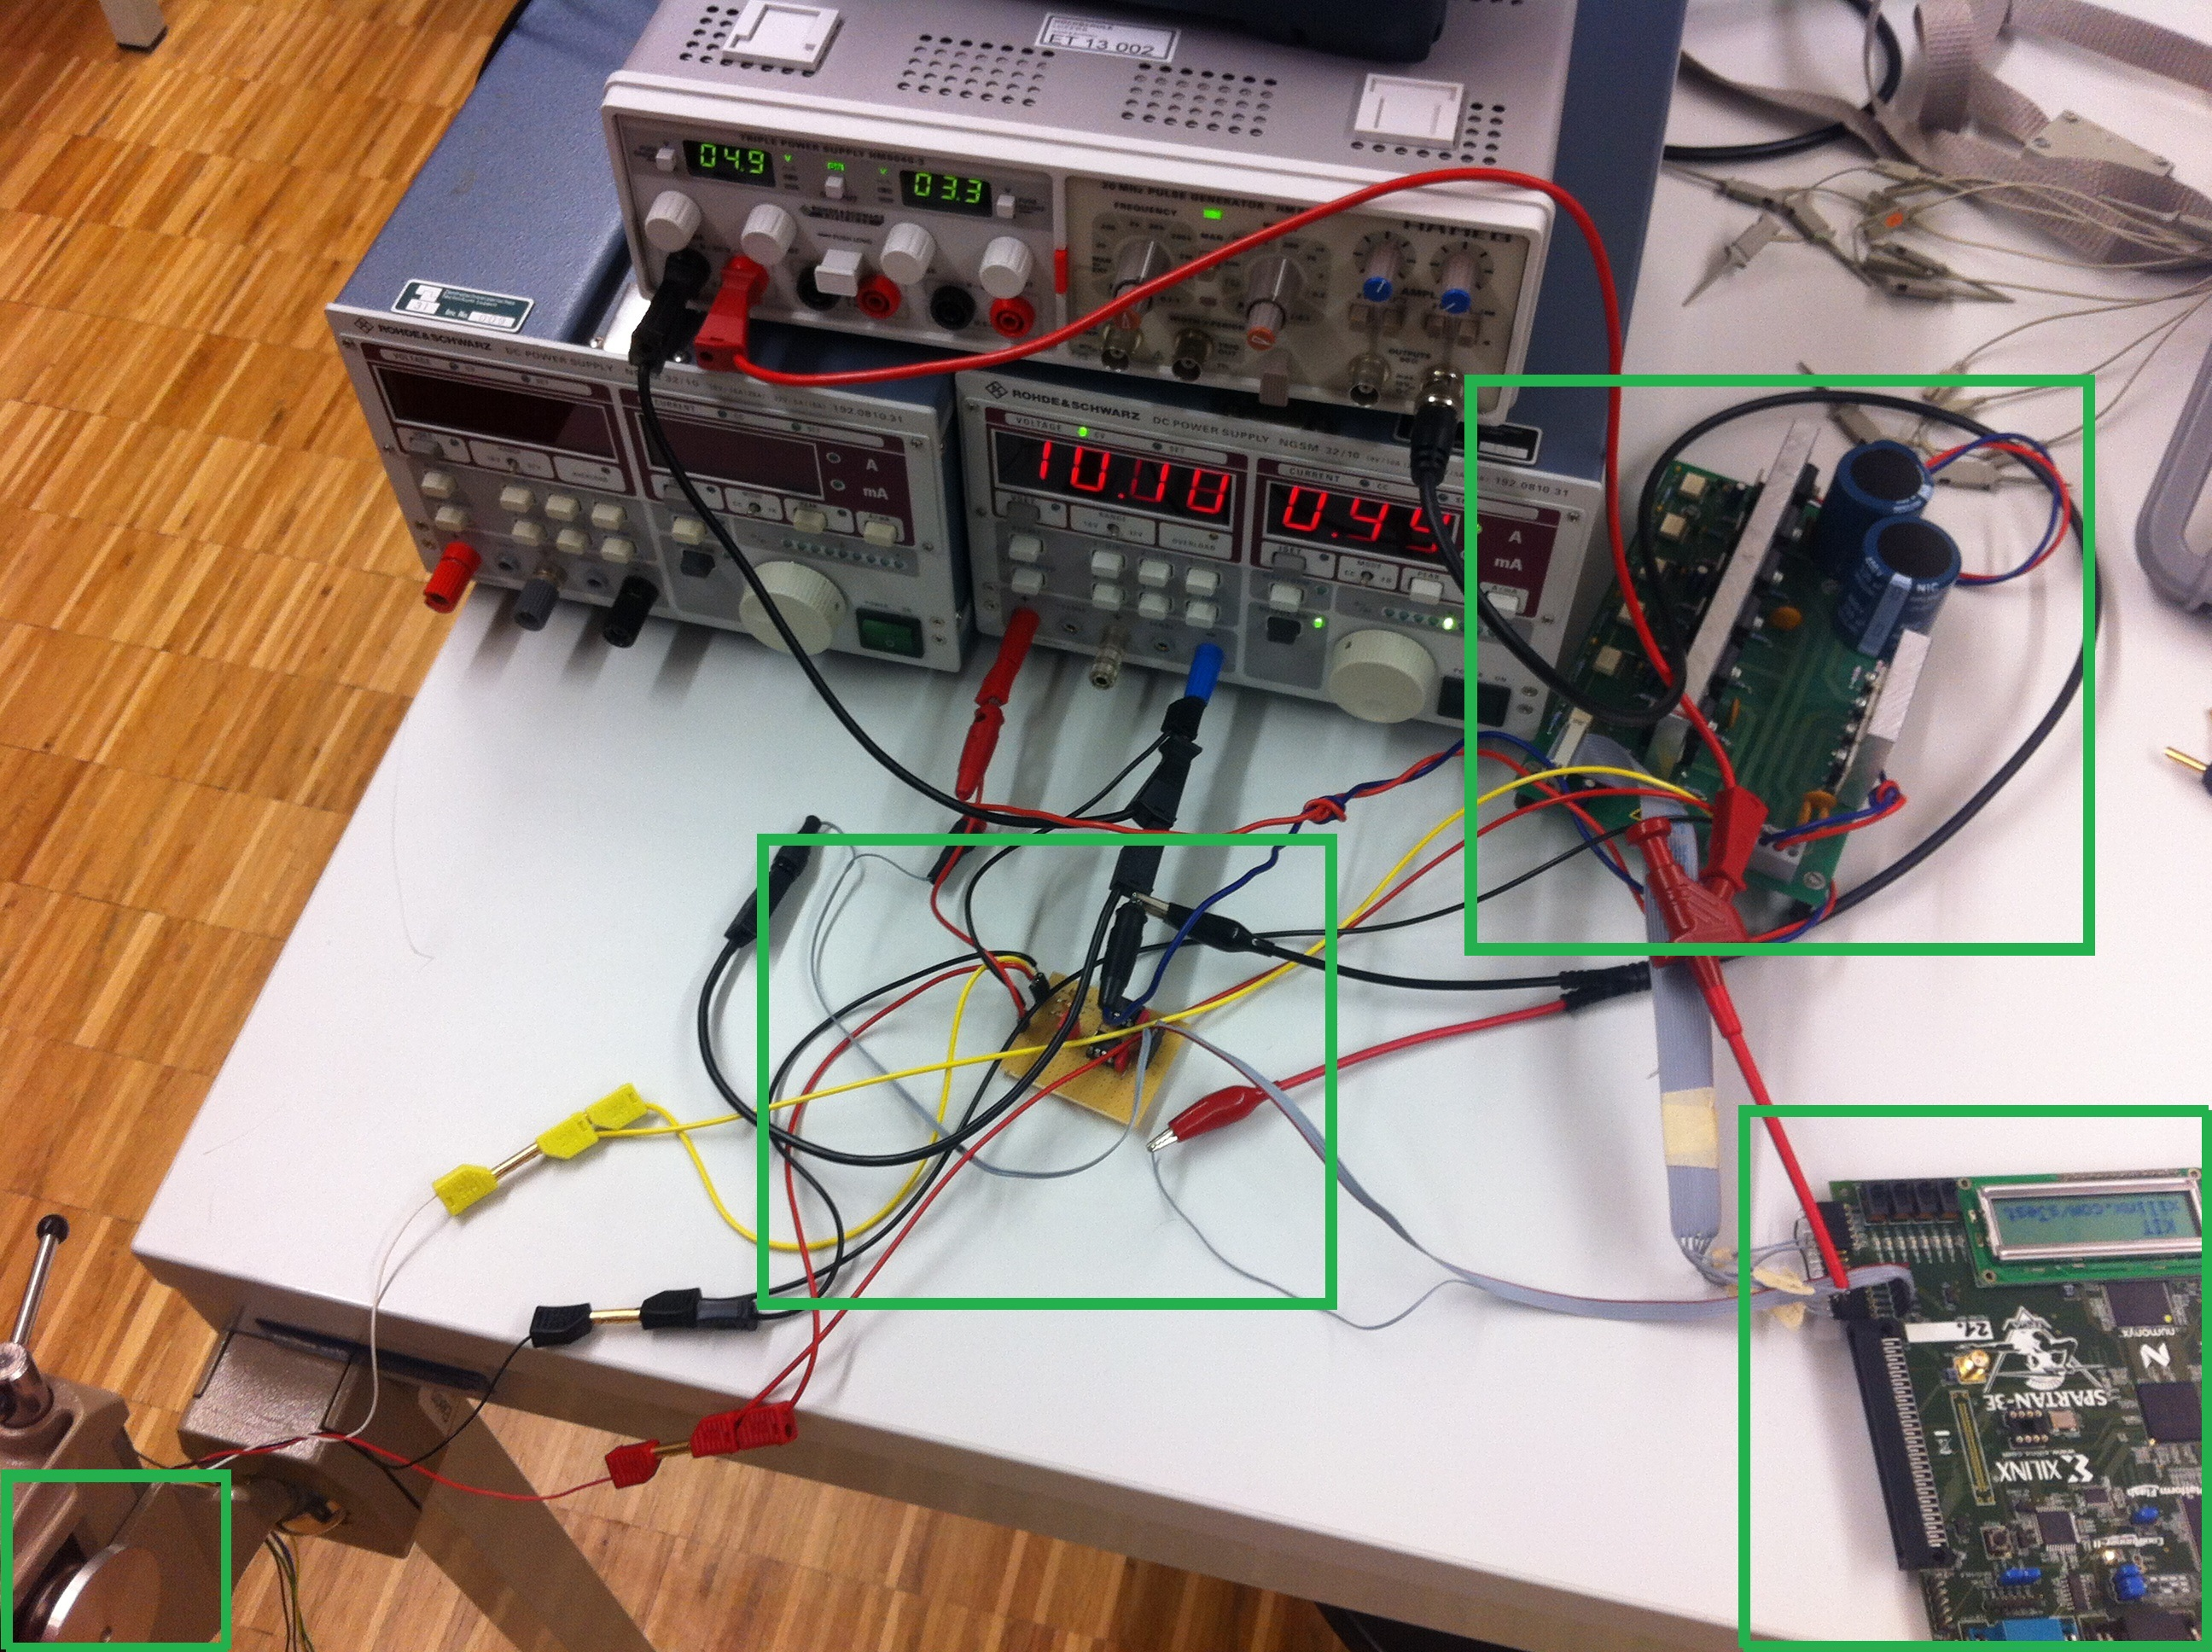
\includegraphics[scale=0.14]{\EtPath/Bilder/MessplatzAufbau.jpg}
       	\centering
       	\caption{Testaufbau} 
        \label{abb:MessplatzAufbau}
    %\vspace{-10pt}
    \end{figure}
    Die im FPGA enthaltene Logik basiert auf der Wahrheitstabelle, die in 
    Abbildung \ref{abb:WahrheitstabelleAnsteuerung} abgebildet ist.

\ifSTANDALONE
\subsection{Messmittel}
\fi
\ifEMBED
\subsubsection{Messmittel}
\fi
    \begin{table}[h!]
        \centering
        \begin{zebratabular}{lll}
            \rowcolor{gray}
            Gerät &
                Typ &
                Nummer \\
            Speisegerät & 
                Rohde \& Schwarz NGSM 32/10 &
                Inv.-Nr. 009 \\
            Oszilloskop &
                Agilent MSO6052A &
                Inv.-Nr. 44; S/N: MY44001903 \\
            Mainframe &
                Hameg HM8001-2 &
                SN: 059520046 \\
            Speisegerät &
                Hameg HM8040-3 &
                SN: 015405014 \\
            Pulsgenerator &
                Hameg HM8035 &
                Inv.-Nr. 44 \\
        \end{zebratabular}
        \caption{Messmittel des Versuchsaufbaus}
    \end{table}

    \clearpage
    \ifSTANDALONE
\section{Fallback}
\fi
\ifEMBED
\subsection{Fallback}
\fi
Ist der Einsatz des vorgesehenen BLDC-Treibers nicht möglich, so muss eine
alternative Ansteuerung erfolgen. Eine solche kann mit einer handelsüblichen
Steuerungen aus dem Modellbau erfolgen. Eine solche BLDC-Steuerung ist per
PWM angesteuert, wobei die im Modellbau üblichen Signale gelten, wie in der
Abbildung \ref{fig:rc-pwm} dargestellt.

\begin{figure}[h!]
	\centering
	\begin{tikzpicture}
		% Achsen
		\draw[->] (-0.25,0) -- (10,0) node[anchor=north] {$t$};
		\draw[->] (0,-0.25) -- (0,3) node[anchor=west] {$u$};
		% Signal
		\draw[-,red,thick] (0,0) -- (1,0) -- (1,2) -- (2,2) -- 
			(2,0) -- (7,0) -- (7,2) -- (8,2) -- (8,0) -- (9,0);
		% Zeiten
		\draw[<->] (1,1.5) -- (7,1.5) node[midway, above] {$T=20$ms};
		\draw[<->] (1,0.5) -- (2,0.5) node[right] {$1$ms$<t_{ON}<2$ms};
	\end{tikzpicture}
	\caption{Signalverlauf eines typischen Modellbau-PWM Signals}
	\label{fig:rc-pwm}
\end{figure}

Der Einsatz von Modellbausteuerungen für BLDC-Motoren erfordert ein
Feedback der Drehzahl, da diese lediglich eine Steuerung darstellen. Die
Drehzahlregelung muss über eine externe Einheit erfolgen, beispielsweise einen
Mikrocontroller. Solche BLDC-Steuerungen werden im Modellbau typischerweise als
\emph{Regler} vertrieben und sind auch für hohe Leistungen durchaus preiswert.

\ifSTANDALONE
\subsection{Konzeptbeschreibung}
\fi
\ifEMBED
\subsubsection{Konzeptbeschreibung}
\fi
Um eine Regelung der Drehzahl des BLDC-Motors zu ermöglichen, bedarf es eines
Feebacks, welches die Drehzahl wiedergibt. Dies ist mit einem
Hall-Effekt-Schalter zu realisieren. Dieser reagiert auf die Magnetfelder,
welche durch Magnete auf dem Rotationskörper gegeben sind. Aus solch einem
Aufbau resultiert ein Feedback, welches mit Impulsen einen Segmentdurchlauf
des Rotationskörpers wiedergibt, wie in Abbildung \ref{fig:fallback-sketch}
dargestellt.
\begin{figure}[h!]
	\centering
	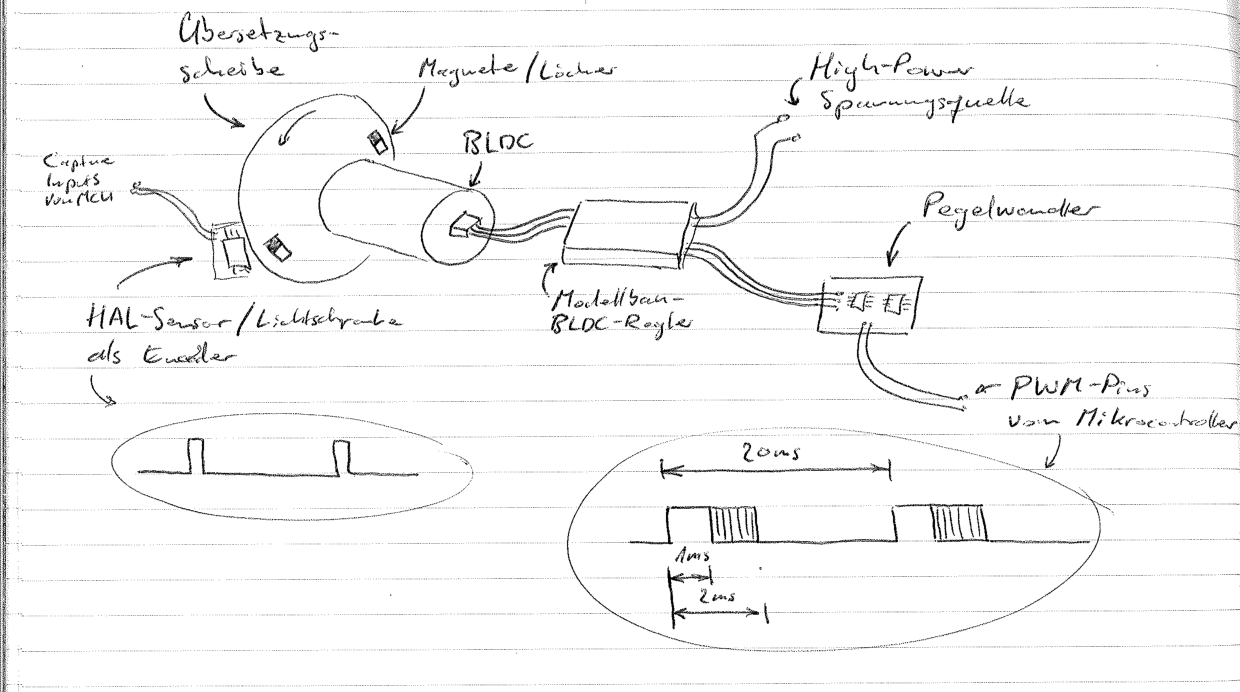
\includegraphics[width=0.8\textwidth]{\EtPath/Bilder/fallback_sketch_1.pdf}
	\caption{Erste Skizze des Fallback-Konzepts}
	\label{fig:fallback-sketch}
\end{figure}
Dieses Feedback wird mittels eines Mikrocontrollers ausgewertet und regelt
damit den Input der Steuerung mit dem PWM-Signal beziehungsweise der Impulsdauer.
Das Einlesen einer Flanke, die Zeitmessung bis zur nächsten Flanke und die
Stellung eines PWM-Signals, sind Tasks welche übliche Mikrocontroller direkt
durch ihre Peripherie-Module ausführen können. Dies ermöglicht eine einfache
Adaption in ein bestehendes Modell, denn es werden lediglich zwei Timer-IO
für diesen Fallback verwendet. Je nach Mikrocontroller ist ein Pegelwandler
für die PWM-Signale notwendig.

    \clearpage
    \ifSTANDALONE
\section{Encoder \& Drehzahlgeber}
\fi
\ifEMBED
\subsubsection{Encoder \& Drehzahlgeber}
\fi

Die vorgesehenen Motorfunktionen verlangen lediglich beim Brushlessmotor
nach einem Feedback über die Rotation des Motors, da der Schrittmotor
definiert und fein granuliert betrieben wird. Der Gleichstrommotor stellt
keinerlei Ansprüche, weder an die Drehzahl, noch an die Position.

Encoder sind relativ teuer und der Einsatz des Brushlessmotors verlangt
lediglich nach einem Feedback zur Rotation beziehungsweise Winkelgeschwindigkeit.
Die absolute oder relative Position ist für die Anwendung nicht von
Bedeutung. Somit lässt sich ein einfaches Feedback vorsehen, für die
Regelung der Drehzahl mit optischen oder magnetischen Elementen.
\ifSTANDALONE
\begin{figure}[h!]
	\centering
	\begin{tikzpicture}
		% Koordinaten
		\draw[->] (-0.5, 0) -- (8, 0) node[anchor=north] {$t$};
		\draw[->] (0, -1.5) -- (0, 3) node[anchor=east] {$u,\varphi$};
		% Rotation
		\draw[blue] (0,0) sin (1,1) cos (2,0) sin (3,-1) cos (4,0)
			sin (5,1) cos (6,0) sin (7,-1)
			node[right] {$\varphi$};
		% Signal
		\draw[-, thick, red]
			(0,0) -- (0.8,0) -- (0.8,2) -- (1.2,2) -- (1.2,0) -- 
			(4.8,0) -- (4.8,2) -- (5.2,2) -- (5.2,0) -- (7.5,0);
		% Messung
		\draw[<->] (0.8,1.5) -- (4.8,1.5) node[midway, above] {$t_{r}$};
	\end{tikzpicture}
	\caption{Vereinfachtes Puls-Feedback eines Hall-Effekt-Schalters}
	\label{fig:hall-effekt-schalter}
\end{figure}
\fi
\ifEMBED
\begin{figure}[h!]
	\centering
	\begin{tikzpicture}
		% Koordinaten
		\draw[->] (-0.5, 0) -- (8, 0) node[anchor=north] {$t$};
		\draw[->] (0, -1.5) -- (0, 3) node[anchor=east] {$u,\varphi$};
		% Rotation
		\draw[blue] (0,0) sin (1,1) cos (2,0) sin (3,-1) cos (4,0)
			sin (5,1) cos (6,0) sin (7,-1)
			node[right] {$\varphi$};
		% Signal
		\draw[-, thick, red]
			(0,0) -- (0.8,0) -- (0.8,2) -- (1.2,2) -- (1.2,0) -- 
			(4.8,0) -- (4.8,2) -- (5.2,2) -- (5.2,0) -- (7.5,0);
		% Messung
		\draw[<->] (0.8,1.5) -- (4.8,1.5) node[midway, above] {$t_{r}$};
	\end{tikzpicture}
	\caption{Vereinfachtes Puls-Feedback eines Hall-Effekt-Schalters}
	\label{fig:hall-effekt-schalter}
\end{figure}
\fi
Als optisches Messinstrument kann eine Lichtschranke mit 
Reflexionsstreifen oder Löchern eingesetzt werden. Diese verlangen
nur nach einer geringfügigen Modifikation des rotierenden Körpers und
sind relativ günstig. Optische Messtechnik hat den Nachteil, das
Störungen relativ leicht in die Messung einfliessen können, was fatale
Folgen für die Regelung hat. Magnetische Messinstrumente sind gegenüber
Störungen deutlich resistenter, da hierfür starke Magnetfelder benötigt
werden, welche so nicht einfach auftreten. Der Einsatz einer solchen Messtechnik
verlangt jedoch nach einer Modifikation der Mechanik, da Magnete in den
rotierenden Körper eingebaut werden müssen. Dies birgt ein gewisses
Risiko für mechanische Unwucht des Rotationskörpers.

\ifSTANDALONE
\subsection{Magnetischer Drehzahlgeber}
\fi
\ifEMBED
\newpage
\paragraph{Magnetischer Drehzahlgeber}$~~$\vspace{2mm}\\
\fi
Um einen eigenen magnetischen Drehzahlgeber zu erstellen wird ein
sogenannter Hall-Effekt-Schalter eingesetzt. Dieser reagiert mit seinem Ausgang
auf ein auftretendes Magnetfeld. Das Gegenstück zum Hall-Effekt-Schalter
ist ein Magnet, welcher in das rotierende Objekt eingebaut wird. Aus 
mechanischen Gründen, wie etwa der Unwucht, werden typischerweise 2 Magnete
oder ein Vielfaches davon in den rotierenden Körper eingebaut.

Bei der Rotation des Körpers entstehen durch das Passieren der Magnete
am Hall-Effekt-Schalter Impulse. Aus diesen Impulsen lässt sich mit einer
Zeitmessung direkt die Drehzahl bestimmen. Die Abbildung 
\ref{fig:hall-effekt-schalter} illustriert das Prinzip anhand eines
Beispiels mit einem Magneten am Rotationskörper.
%
\ifSTANDALONE
\begin{figure}[h!]
	\centering
	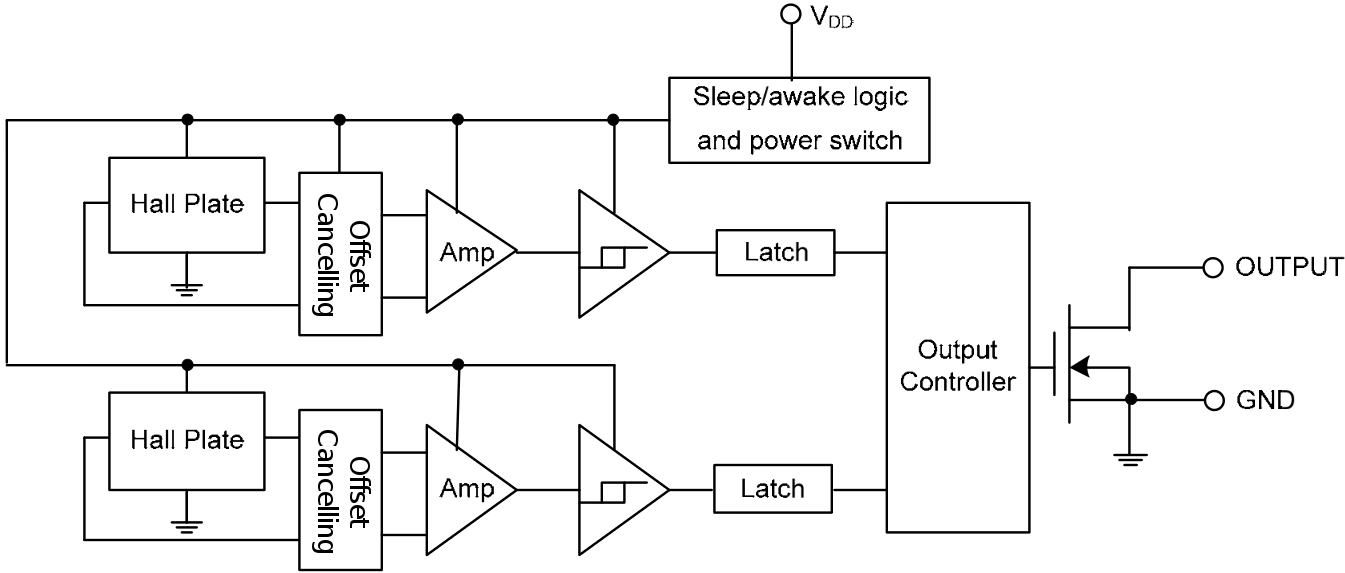
\includegraphics[width=0.75\textwidth]{\EtPath/Bilder/AH180N_functional.png}
	\caption{Funktionelles Blockschaltbild des Hall-Effekt-Schalters AH180N}
	\label{fig:AH180N_functional}
\end{figure}
\fi
%
\ifEMBED
\begin{figure}[h!]
	\centering
	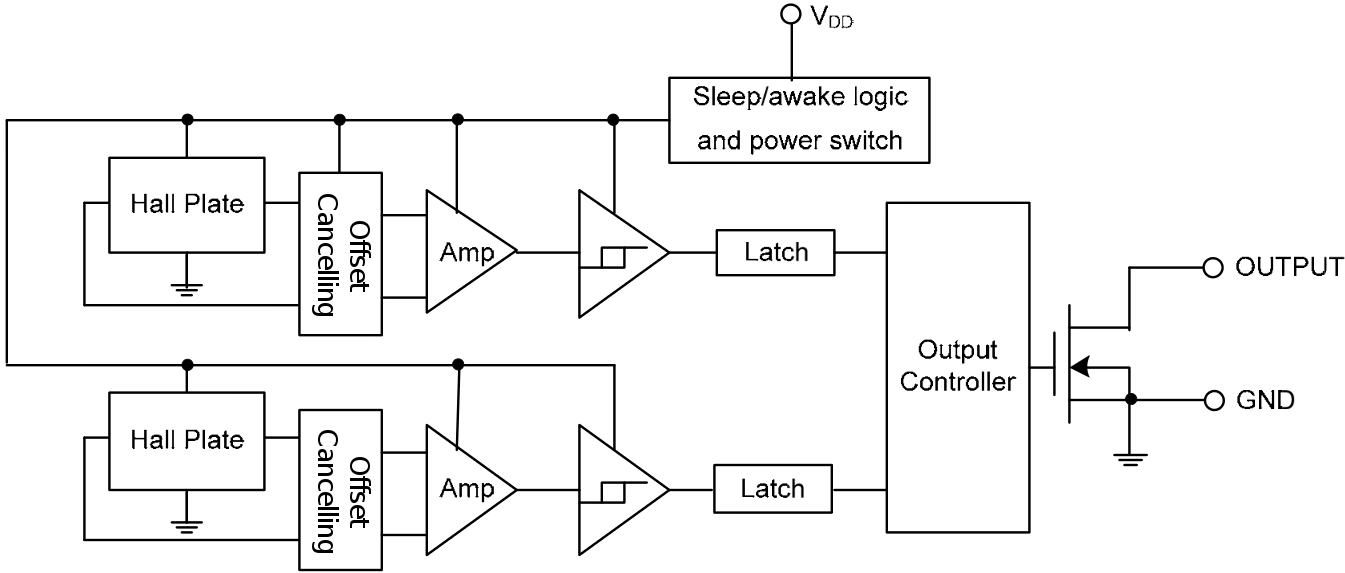
\includegraphics[width=0.75\textwidth]{\EtPath/Bilder/AH180N_functional.png}
	\caption{Funktionelles Blockschaltbild des Hall-Effekt-Schalters AH180N}
	\label{fig:AH180N_functional}
\end{figure}
\fi
%
Ein solches Verfahren lohnt sich bei schnellen Winkelgeschwindigkeiten
und ist für diesen Anwendungsfall sehr effizient. Zugehörige
Hall-Effekt-Schalter lassen sich einfach montieren und sind gegen Störungen
sehr robust. Ein mögliches Modell für einen Hall-Effekt-Schalter ist der
AH180N. Dieser bietet einen Open-Drain Ausgang, welcher somit logische Pegel
liefert (siehe Abbildung \ref{fig:AH180N_functional}). Interessant ist diese
Art von Drehzahl-Geber insbesondere durch ihren geringen Preis, denn solche
Hall-Effekt-Schalter, wie der AH180N, befinden sich im Preissegment von 
unter einem Franken.
    \clearpage
\fi

\ifSTEPPER
    \renewcommand{\EtPath}{src/Stepper}
    \ifSTANDALONE
\section{Wirkungsweise} \label{wirkungsweise}
\fi
\ifEMBED
\subsection{Wirkungsweise} \label{wirkungsweise}
\fi

\ifEMBED
    % Dieses Kapitel ist eine Zusammenarbeit der Gruppen \BLDCTeams. 
    \BLDCcollab
\fi
    
    Schrittmotoren oder auch Stepper genannt, sind Synchronmotoren, bei 
    welchen der Rotor um einen bestimmten Winkel gedreht werden kann. So ist 
    die Rotorposition ohne zusätzliche Sensoren bekannt. Dabei ist zu 
    beachten, dass der Motor keine Schritte verliert, was bei Überlast 
    geschehen kann. Da die meisten Schrittmotorensysteme Open- Loop Systeme 
    sind, entsteht eine dauernde Positionsabweichung bei einem Schrittverlust. 
    Grundsätzlich wird zwischen zwei Schrittmotortypen unterschieden: 
    \begin{itemize}
       	\item Permagnentmagnetmotor
       	\item Reluktanzmotor
    \end{itemize} 
    Der Permanentmagnetmotor besitzt als Rotor einen Permagnentmagneten. Beim 
    Reluktanzmotor besteht der Rotor aus einem gezahnten Weicheisenkern. 
    Permanentmagnetmotoren erreichen eine kleinere Schrittfrequenz, besitzen 
    jedoch ein grösseres Drehmoment als der Reluktanzmotor. Die Kombination 
    aus Reluktanzmotor und Permanentmagnetmotor ist ein Hybridmotor. Ein 
    Hybridmotor verbindet die Vorteile von Reluktanz- und Permagnentmotor.
    
    Der Vollschrittbetrieb kann einphasig oder auch zweiphasig gesteuert 
    werden. Beim einphasigen Vollschrittbetrieb sind immer zwei gegenüber 
    liegende Pole aktiv. Beim zweiphasigen Vollschrittbetrieb werden jeweils 
    zwei nebeneinander liegende Pole aktiv. Im Halbschrittbetrieb werden die 
    beiden Vollschrittbetriebsarten kombiniert. So kann der Schrittwinkel 
    halbiert werden. Zusätzlich kann der Schrittmotor mit Mikroschritten 
    betrieben werden. Dabei folgt der Strom der sinusförmigen 
    Referenzspannung. (Vgl. Seite \pageref{stromgesteuert})
    \begin{figure}[H]
    	\centering
    	\begin{tikzpicture}
        % Hilfslinien
        \foreach \i in {0, 0.5, ..., 4.5}
        {
            \draw[ultra thin, gray] (\i, 1.9) -- (\i, -0.7);
        }
        % Achsen
    	\draw[->]	(0, 0) -- (0, 2);
    	\draw[->]	(0, 1.2) -- (5, 1.2) node[right]{A};
    	\draw[->]	(0, 0) -- (5, 0) node[right]{B};
        % Kurven
        \draw[red] 
            (0     ,0.7) --
            (0.5   ,0.7) --
            (0.5   ,1.2) --
            (1     ,1.2) --
            (1     ,1.7) --
            (1.5   ,1.7) --
            (1.5   ,1.2) --
            (2     ,1.2) --
            (2     ,0.7) --
            (2.5   ,0.7) --
            (2.5   ,1.2) --
            (3     ,1.2) --
            (3     ,1.7) --
            (3.5   ,1.7) --
            (3.5   ,1.2) --
            (4     ,1.2) --
            (4     ,0.7) --
            (4.5   ,0.7);
        \draw[red] 
            (0      ,0) --
            (0.5    ,0) --
            (0.5    ,0.5) --
            (1      ,0.5) --
            (1      ,0) --
            (1.5    ,0) --
            (1.5    ,-0.5) --
            (2      ,-0.5) --
            (2      ,0) --
            (2.5    ,0) --
            (2.5    ,0.5) --
            (3      ,0.5) --
            (3      ,0) --
            (3.5    ,0) --
            (3.5    ,-0.5) --
            (4      ,-0.5) --
            (4      ,0) --
            (4.5    ,0) ;
    	\end{tikzpicture}
    	\caption{Vollschritt}
    	\label{fig:vollschritt}
    \end{figure}
    
    \begin{figure}[H]
     	\centering
     	\begin{tikzpicture}
        % Hilfslinien
        \foreach \i in {0, 0.25, ..., 4.5}
        {
            \draw[ultra thin, gray] (\i, 1.9) -- (\i, -0.7);
        }
        % Achsen
    	\draw[->]	(0, 0) -- (0, 2);
    	\draw[->]	(0, 1.2) -- (5, 1.2) node[right]{A};
    	\draw[->]	(0, 0) -- (5, 0) node[right]{B};
        % Kurven
        \draw[red] 
            (0     ,0.7) --
            (0.75   ,0.7) --
            (0.75   ,1.2) --
            (1     ,1.2) --
            (1     ,1.7) --
            (1.75   ,1.7) --
            (1.75   ,1.2) --
            (2     ,1.2) --
            (2     ,0.7) --
            (2.75   ,0.7) --
            (2.75   ,1.2) --
            (3     ,1.2) --
            (3     ,1.7) --
            (3.75   ,1.7) --
            (3.75   ,1.2) --
            (4     ,1.2) --
            (4     ,0.7) --
            (4.5   ,0.7);
        \draw[red] 
            (0      ,-0.5) --
            (0.25   ,-0.5) --
            (0.25   ,0) --
            (0.5    ,0) --
            (0.5    ,0.5) --
            (1.25   ,0.5) --
            (1.25   ,0) --
            (1.5    ,0) --
            (1.5    ,-0.5) --
            (2.25   ,-0.5) --
            (2.25   ,0) --
            (2.5    ,0) --
            (2.5    ,0.5) --
            (3.25   ,0.5) --
            (3.25   ,0) --
            (3.5    ,0) --
            (3.5    ,-0.5) --
            (4.25   ,-0.5) --
            (4.25   ,0) --
            (4.5    ,0) ;
     	\end{tikzpicture}
     	\caption{Halbschritt}
     	\label{fig:halbschritt}
    \end{figure}
    \begin{figure}[H]
    	\centering
    	\begin{tikzpicture}
        % Hilfslinien
        \foreach \i in {0, 0.05, ..., 4.5}
        {
            \draw[ultra thin, gray] (\i, 1.9) -- (\i, -0.7);
        }
        % Achsen
    	\draw[->]	(0, 0) -- (0, 2);
    	\draw[->]	(0, 1.2) -- (5, 1.2) node[right]{A};
    	\draw[->]	(0, 0) -- (5, 0) node[right]{B};
        % Kurven
        \foreach \i in {0, 0.05, ..., 4.5}
        {
            \draw[red] (\i, {0.5*sin(180*\i)})          -- (\i+0.05, {0.5*sin(180*\i)});
            \draw[red] (\i, {0.5*sin(180*\i+(90))+1.2}) -- (\i+0.05, {0.5*sin(180*\i+(90))+1.2});
        }
    	\end{tikzpicture}
    	\caption{Mikroschritt}
    	\label{fig:mikroschritt}
    \end{figure}
    Eine Phase sind jeweils die zusammengeschalteten Statorwicklungen. Der 
    unipolare Schrittmotor besteht aus vier Phasen. Ein Elektromagnet besteht 
    aus zwei Phasen, welche gegenseitig gewickelt sind. So kann vermieden 
    werden, dass der Stromfluss durch die Wicklung gedreht werden muss. Der 
    Bipolare Schrittmotor besteht aus nur zwei Phasen. Es muss mit einer 
    Brückenschaltung die Richtung des Stromes gedreht werden. In den meisten 
    Anwendungen werden Bipolare Schrittmotoren verwendet, da ein bipolarer 
    Schrittmotor ein grössseres Drehmoment erzeugt als ein gleich grosser 
    unipolarer Schrittmotor. Die beiden Betriebsarten sind in der 
    \autoref{fig:uniVsbi} ersichtlich. 
    \begin{figure}[H]
       	\centering
       	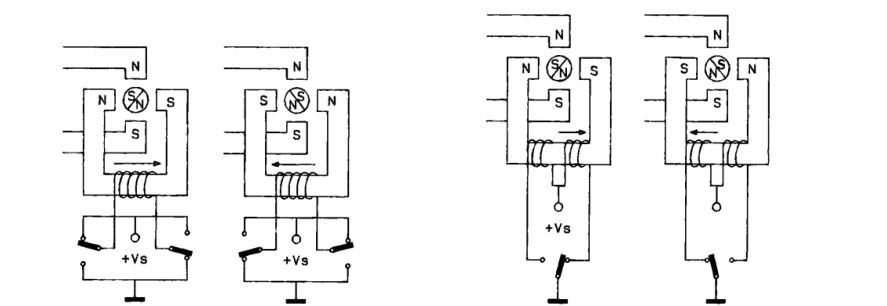
\includegraphics[width=12cm]{\EtPath/Bilder/uniVsbi.jpg}
       	\caption{bipolarer und unipolarer Betrieb}
       	\label{fig:uniVsbi}
    \end{figure}
    
       
    

    \clearpage
    \ifSTANDALONE
\section{Stepper Motoransteuerung}
\fi
\ifEMBED
\subsection{Stepper Motoransteuerung}
\fi

\ifEMBED
    % Dieses Kapitel ist eine Zusammenarbeit der Gruppen \BLDCTeams. 
    \BLDCcollab
\fi
    \ifSTANDALONE
    \subsection{Grundsätzliches zur Ansteuerung}\label{subsec:Ansteuerung}
    \fi
    \ifEMBED
    \subsubsection{Grundsätzliches zur Ansteuerung}\label{subsec:Ansteuerung}
    \fi
    	Grundsätzlich besteht die Ansteuerung aus drei Teilen, wie in \autoref*{fig:ansteuerung} gezeigt. 
    	\begin{figure}[H]
    		\centering
    		\begin{tikzpicture}
    		\draw[line width=1.5pt](0, 0) rectangle node{Mikrokontroller} (3, 1)  ;
    		\draw[line width=1.5pt, ->]	(3, 0.5) -- (4, 0.5);
    		\draw[line width=1.5pt](4, 0) rectangle node{Steuerung}(7, 1);
    		\draw[line width=1.5pt, ->]	(7, 0.5) -- (8, 0.5);
    		\draw[line width=1.5pt](8, 0) rectangle node{Treibertufen}(11, 1);
    		\end{tikzpicture}
    		\caption{Komponenten der Ansteuerung eines Schrittmotores}
    		\label{fig:ansteuerung}
    	\end{figure}
        Um die Ansteuerung zu realisieren, gibt es eine Vielzahl von integrierten Schaltkreisen. Diese unterscheiden sich wie folgt: 
        \begin{itemize}
        	\item \textbf{Interfaces:} Einzelanschlüsse, einfache Busschnittstellen oder Mikrokontrollerschnittstellen wie SPI, II2
        	\item \textbf{Steuerfunktionen:} Einzelne Schritte oder Bewegungsabläufe (Motion Control Functiona)
        	\item \textbf{Schaltungsintegration:} Steuerung und Treiberstufe als getrennte Schaltkreise, oder in einem Schaltkreis zusammengefasst. 
        \end{itemize}
        Der gewählte integrierte Schaltkreis ist der L6480 von STMicroelectronics. Dieser wird über die SPI Schnittstelle gesteuert und besitzt eine Motion Contol Engine. Die Treiberstufe wird extern realisiert. (Vgl. Kapitel \ref{sec:L6480} 
        
    \ifSTANDALONE
    \subsection{Treiberstufe}
    \fi
    \ifEMBED
    \subsubsection{Treiberstufe}
    \fi 
    	Wird ein Schrittmotor unipolar betrieben, so können die vier Wicklungen direkt mit Leistungsstufen angesteuert werden. Für den bipolaren Betrieb benötigt man für beide Wicklungen je eine H- Brücke. Die einfachste Methode ist es, den Strom nur durch den Wicklungswiderstand zu begrenzen. Der Nachteil ist, dass die Zeitkonstante durch den Wicklungswiderstand und der Induktivität bestimmt ist, und so bei höheren Schrittfrequenzen der gewünschte Strom und damit das Drehmoment nicht mehr erreicht wird. Deshalb wird ein zusätzlicher Vorwiderstand in Serie geschaltet, und so die Zeitkonstante verkleinert. Typische Verhältnisse sind vierfacher- oder fünffacher Widerstand, was eine vierfache bzw. fünffache Speisespannung voraussetzt. Diese Methode wiederum führt zu einer höheren Verlustleistung in den Widerständen. Im Ruhezustand ist es sinnvoll, den Strom soweit zu senken, dass das Haltemoment nicht unterschritten wird. Eine Spannungsumschaltung hat den weiteren Vorteil, dass so beim Anfahren eine steilere Stromkurve erreicht werden kann. (Vgl. \autoref{fig:spannungsumschaltung})
    	 \begin{figure}
    	 	\centering
    	 	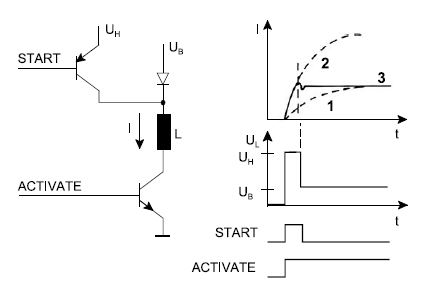
\includegraphics[width=8cm]{\EtPath/Bilder/spannungsumschaltung.JPG}
    	 	\caption{Spannungsumschaltung}
    	 	\label{fig:spannungsumschaltung}
    	 \end{figure}
    	Der Schrittmotor kann alternativ auch stromgesteuert betrieben werden. Dabei folgt der Stromverlauf dem Verlauf einer Referenzspannung (Sollwert). Der Stromverlauf wird auf den Sollwert geregelt. Die Betriebsspannung muss so nicht stabilisiert werden. \label{stromgesteuert} 
	
	
		
    \clearpage
    \ifSTANDALONE
    \section{Stepper Driver L6480} \label{sec:L6480}
\fi
\ifEMBED
    \subsection{Stepper Driver L6480} \label{sec:L6480}
\fi
\ifEMBED
    % Dieses Kapitel ist eine Zusammenarbeit der Gruppen \BLDCTeams. 
    \BLDCcollab
\fi
Wie bereits im Kapitel \ref*{subsec:Ansteuerung} erwähnt, wird der L6480 von STMicroelectronics verwendet. 

\ifSTANDALONE
    \subsection{Funktionsbeschreibung}
\fi
\ifEMBED
    \subsubsection{Funktionsbeschreibung}
\fi
    Diese Schrittmotorensteuerung ist für den Betrieb von zweiphasigen (Vgl. 
    Kpaitel \ref{wirkungsweise}) Schrittmotoren mit Mikrosteps (Vgl. Kapitel 
    \ref{wirkungsweise}) geeignet. Der L6480 erreicht eine maximale Auflösung 
    von einem 1/128 Schritt. Die Steuerung generiert intern die PWM- Signale 
    für die Motorenansteuerung. Alternativ kann auch mit Vollschritten oder 
    Halbschritten gearbeitet werden. Die beiden H- Brücken werden extern mit 
    N-Kanal MOSFETs realisiert. Es können Bewegungsprofile konfiguriert 
    werden, so dass die Motoren definiert anfahren, abbremsen oder ein Punkt 
    direkt angefahren werden kann. So kann der Aufwand bei der 
    Mikrocontrollerprogrammierung verringert werden. Die Befehle werden über 
    eine SPI- Schnittstelle übertragen. Die absolute Position ist in einem 22- 
    Bit Register gespeichert. Der Bereich liegt dementsprechend zwischen 
    \(-2^{21}\) und \(2^{21}-1\). \cite{Datasheet:L6480} 

\ifSTANDALONE
    \subsection{Schnitstelle}
\fi
\ifEMBED
    \subsubsection{Schnittstelle}
\fi
Der steuernde Mikrocontroller benötigt 8 Pins für die Kommunikation mit dem 
L6480 \cite{Datasheet:L6480} : 
\begin{table}[h!]
    \begin{zebralongtable}{l l p{7cm}}
        \rowcolor{gray}\textbf{Pin} &
            \textbf{IO} &
            \textbf{Funktion} \\
        $\overline{FLAG}$ &
            Output (Open Drain) &
            Wird bei einem Fehler intern auf GND gezogen. \\
        $\overline{BUSY}$ / SYNC &
            Output (Open Drain) &
            Wird während dem Ausführen eines Befehls intern auf GND gezogen.\\
        $\overline{STBY / RESET}$ &
            Input &
            Standby- und Resetmodus, falls extern GND anliegt. \\
        STCK &
            Input &
            Im Step-Clock- Mode führt jede positive Flanke an diesem Pin zu einem 
                Schritt. \\
        \rowcolor{gray}\textbf{SPI} & & \\
        $\overline{CS}$ &
            Input &
            Chip Select: Falls extern GND anliegt, startet die Kommunikation. Um 
                die Kommunikation zu beenden, muss $\overline{CS}$ extern auf High 
                gehalten werden. \\
        CK &
            Input &
            Serial Clock: Synchronisierung der Kommunikation. \\
        SDO &
            Output &
            Slave Data Out: Daten für den Mikrocontroller. \\
        SDI &
            Input &
            Slave Data In: Befehle und Daten für den L6480. \\
    \end{zebralongtable}
    \caption{Schnittstelle des Treibers L6480}
    \label{Schnittstelle}
\end{table}
%\begin{longtable}{l l p{7cm}} \toprule
%    \textbf{Pin}    & \textbf{IO}   & \textbf{Funktion} \\
%    \midrule
%    \endhead
%    \multicolumn{3}{l}{\emph{Fortsetzung auf nächster Seite}} \\ \bottomrule \endfoot \endlastfoot          
%    \textbf{IO}\\ \addlinespace
%    %\cmidrule{1-1}
%    $\overline{FLAG}$& Output               & Wird bei einem Fehler intern auf GND gezogen. \\ \addlinespace
%    $\overline{BUSY}$ / SYNC & Output       & Wird während dem Ausführen eines Befehls intern auf GND gezogen.\\ \addlinespace
%    $\overline{STBY / RESET}$& Input        & Standby- und Resetmodus, falls extern GND anliegt. \\ \addlinespace
%    STCK            & Input         & Im Step-Clock- Mode führt jede positive Flanke an diesem Pin zu einem Schritt. \\ \addlinespace
%    %\cmidrule{1-1}
%    \textbf{SPI}\\ \addlinespace
%    %\cmidrule{1-1}
%    $\overline{CS}$ & Input         & Chip Select: Falls extern GND anliegt, startet die Kommunikation. Um die Kommunikation zu beenden, muss $\overline{CS}$ extern auf High gehalten werden. \\ \addlinespace
%    CK              & Input         & Serial Clock: Synchronisierung der Kommunikation. \\ \addlinespace
%    SDO             & Output        & Slave Data Out: Daten für den Mikrocontroller. \\ \addlinespace
%    SDI             & Input         & Slave Data In: Befehle und Daten für den L6480. \\ \addlinespace
%    \bottomrule
%    \\
%    \caption{Schnittstelle} 
%    \label{Schnittstelle}
%\end{longtable} 

\ifSTANDALONE  
    \newpage 
    \subsection{Typical Application}
\fi
\ifEMBED
    \subsubsection{Typical Application}
\fi
\begin{figure}[h]
    \centering
    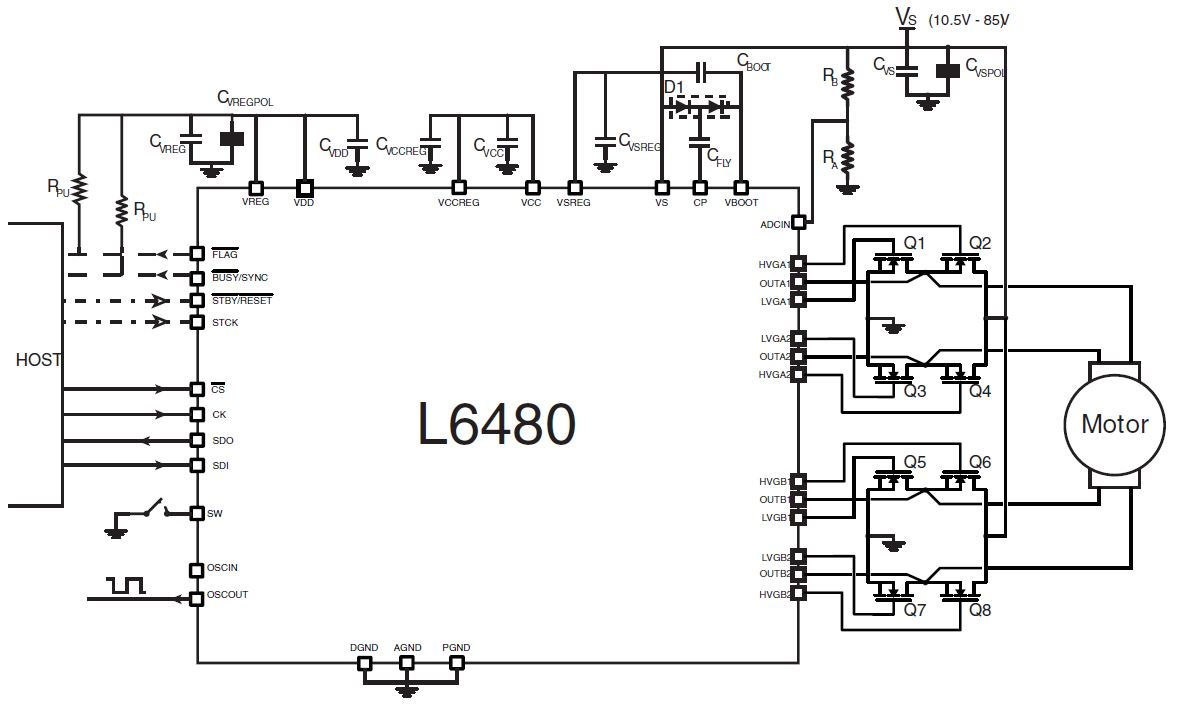
\includegraphics[width=12cm]{\EtPath/Bilder/typicalApp.jpg}
    \label{fig:typApp}
    \caption[Typical Application]{Typical Application \cite{Datasheet:L6480}}
\end{figure}

    \clearpage
    \ifSTANDALONE
\section{Ausblick}
\fi
\ifEMBED
\subsection{Ausblick}
\fi
	In einem nächsten Schritt soll der L6480 bestellt werden und in einer Testschaltung getestet werden. Weiter soll ein Schema und ein Layout geplant und produziert werden, welche alle Teammitglieder in ihrem Projekt verwenden können, falls sie dies benötigen. 
    \clearpage
\fi

\setlength\bibitemsep{1.5\itemsep}
%Folgende Zeile auskommentieren, damit nur gebrauchte Literatur erscheint
%\nocite{*}
\renewcommand{\refname}{Literatur- und Quellenverzeichnis}
% \bibliographystyle{apacite} set in layout.sty -> do not try to set it here again!
\bibliography{\BIBLIOGRAPHY}

\listoffigures
\listoftables
